% !TEX root = main.tex

\newcommand{\code}[1]{\texttt{#1}}
\newcommand{\ddash}{-{}-}
\newcommand{\eg}{e.g.}
\newcommand{\ie}{i.e.}
\newcommand{\vs}{vs.}

\graphicspath{{fig/}, {images/}}

\title{Version control with \texttt{git} --- why? what? how?}
%\subtitle{Just a subtitle}
\date{February 17, 2022}
\author[Matthias Mayr]{Matthias Mayr \inst{1,2}}
\institute[Universität der Bundeswehr München]{
\inst{1} Institute for Mathematics and Computer-Based Simulation, Universität der Bundeswehr München
\and
\inst{2} Data Science \& Computing Lab, Universität der Bundeswehr München
}
\event{CompSim@IMCS Group Meeting}
\eventdetails{Institute for Mathematics and Computer-Based Simulation\\Department for Civil Engineering and Environmental Sciences\\February 17, 2022}
\titlegraphic{\centering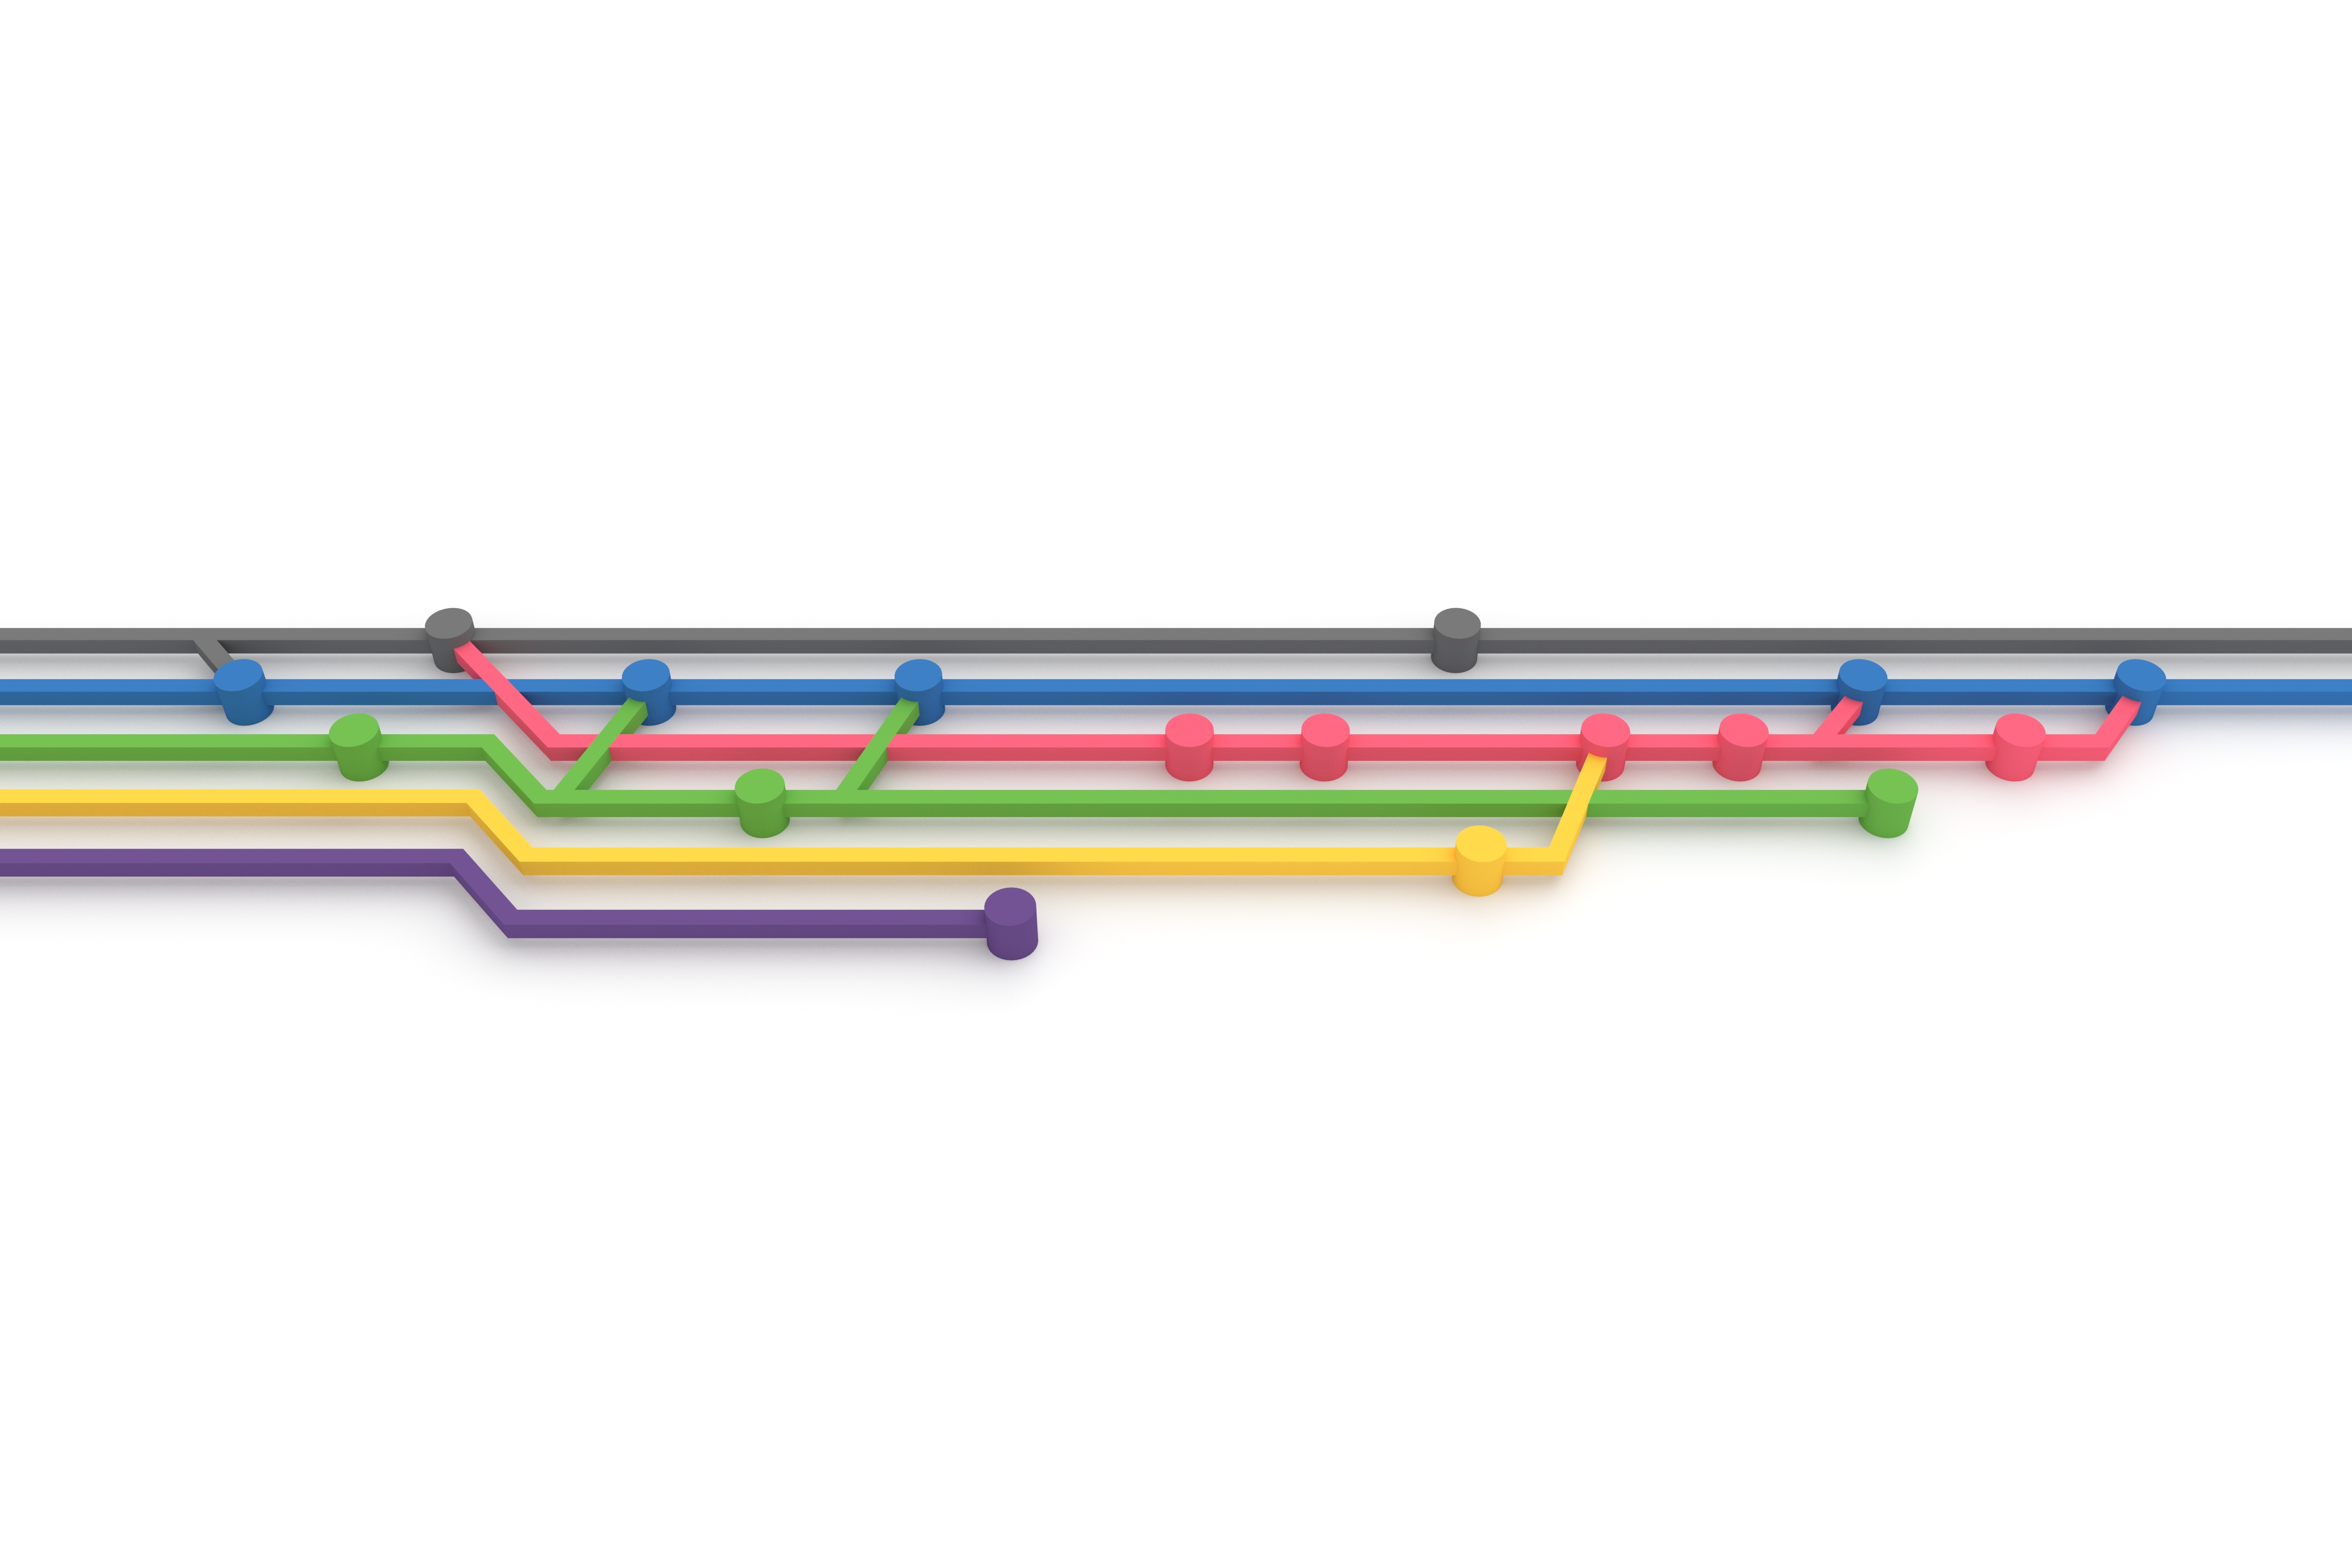
\includegraphics[width=\slidewidth,trim={0, 8cm, 0, 8cm},clip]{images/git_branches.jpeg}}

% All Baci-related info is wrapped into this command, so that it can be dumped to nowhere for non-Baci talks.
%\newcommand{\baci}[1]{#1}
\newcommand{\baci}[1]{}

\usepackage[backend=bibtex]{biblatex}
\bibliography{bibliography}

%\usepackage{bibentry}
%\nobibliography*

\begin{document}

\begin{frame}[plain,noframenumbering]
\titlepage
\end{frame}

\begin{frame}{Disclaimer}
\begin{columns}
\column{0.5\textwidth}
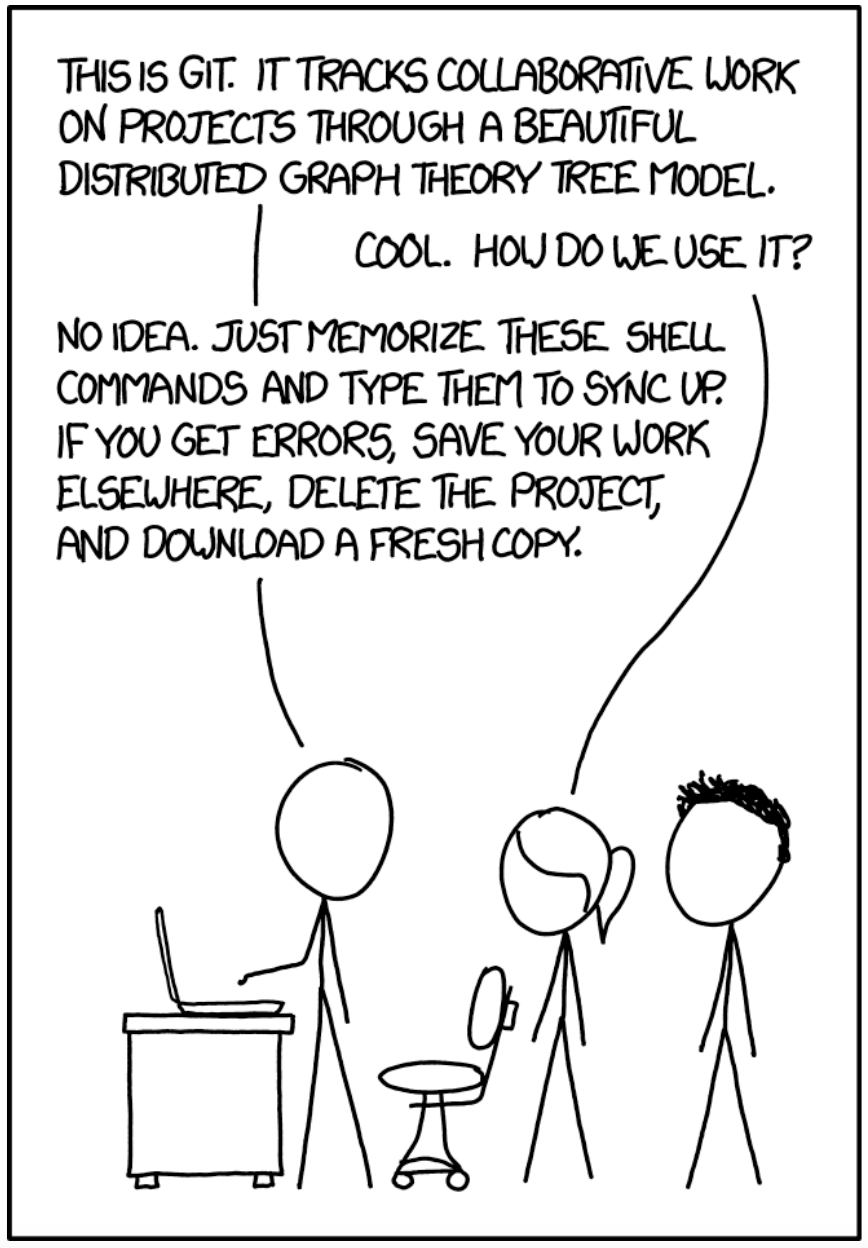
\includegraphics[width=\columnwidth]{images/xkcd_git.png}
\column{0.5\textwidth}
\begin{itemize}
\item This is just a quick overview of basic ideas and commands, not a tutorial.
\item Best way to learn \code{git}: use it every day!
\item For help, consult either the internet or your colleagues.
\end{itemize}
\end{columns}
\end{frame}

\begin{frame}{Agenda}
\tableofcontents
\end{frame}

\section{Some thoughts on using \texttt{git}}

\begin{frame}{Why \code{git} for day-to-day software development?}
\begin{columns}
\column{0.8\textwidth}
\begin{itemize}
\item \structure{Version control}: tracking every change to the source code as snapshots / \structure{commit}
\item \structure{Independent} development by multiple developers
\item Always one branch ready to deploy: \code{main}
\item Share work among developers for collaborative software development
\end{itemize}
\column{0.2\textwidth}

\includegraphics[width=\columnwidth]{images/logo_git.png}
\end{columns}

\vspace{1em}
\textbf{Remarks:}
\begin{itemize}
\item Previously, the default branch was called \code{master}. Remember: it is just a name, so one can easily rename it, {\eg} to \code{main}.
\end{itemize}

\begin{block}{\code{git} for source code, but for what else?}
\code{git} can be used for any \code{ASCII}-based files, {\eg} \LaTeX, Markdown, ...
\end{block}
\end{frame}

\begin{frame}{What should I keep in mind when using \code{git}?}
\begin{itemize}
\item Write \structure{meaningful commit messages}\footnote{\scriptsize{\url{https://tbaggery.com/2008/04/19/a-note-about-git-commit-messages.html}}}
\begin{itemize}
\item First line: capitalized, short commit summary (max. 50 characters)
\item Second line: empty
\item Body (w/ max. 72 characters per line) to describe the reasoning behind the proposed changes (``What \& Why?'').
\begin{itemize}
\item Use imperative.
\item Focus on the ``What \& Why?''. The ``How?'' how can be seen from the proposed changes.
\item Use empty lines to separate paragraphs.
\item Maybe include references to issue tracker or merge/pull requests.
\end{itemize}
\end{itemize}
\item Each commit should compile w/o errors.
\item Aim for a \structure{clean} history.
\end{itemize}
\end{frame}

\section{The concept of \code{git}}

\begin{frame}{Working with branches}
\begin{columns}[T]
\column{0.49\textwidth}
\begin{itemize}
\item The \structure{\code{main}} branch is always clean, stable, and deployable.
\item Actual development work happens on \structure{feature branches}.
\item<2-> Create a new branch via \code{git checkout -b <branchName>}
\item<3-> Do all your work and commits on this feature branch \code{<branchName>}
\item<4-> When done, bring changes to the \code{main} branch
\end{itemize}
\column{0.49\textwidth}
\begin{block}{Branches}
\centering
\begin{tikzpicture}[
scale=0.8,
node distance=0.7cm,
nodestyle/.style={draw,thick,circle},
edgestyle/.style={thick}
]
\node[text=colorMain!50,rotate=90] at (1.0cm,0.0cm) {\code{main}};
\onslide<1-3>{
\draw[thick,dashed,fill=colorMain!50,rounded corners=3pt] (-0.55cm,-0.55cm) rectangle (0.55cm,2.3cm);
}
\onslide<4>{
\draw[thick,dashed,fill=colorMain!50,rounded corners=3pt] (-0.55cm,-0.55cm) rectangle (0.55cm,4.0cm);
}
\onslide<5>{
\draw[thick,dashed,fill=colorMain!50,rounded corners=3pt] (-0.55cm,-0.55cm) rectangle (0.55cm,5.7cm);
}

\onslide<2->{
\node[text=colorSec!50,right,rotate=90] at (2.2cm,2.2cm) {\code{<branchName>}};
}
\onslide<2>{
\draw[thick,dashed,fill=colorSec!50,rounded corners=3pt] (0.65cm,2.4cm) rectangle (1.75cm,3.4cm);
}
\onslide<3->{
\draw[thick,dashed,fill=colorSec!50,rounded corners=3pt] (0.65cm,2.4cm) rectangle (1.75cm,7.0cm);
}

\node[nodestyle] (A) at (0,0) {A};
\node[nodestyle,above=of A] (B) {B};
\draw[edgestyle] (A) -- ++(0,-0.7cm);
\draw[edgestyle] (A) -- (B);

\onslide<2->{
\node[nodestyle,above right=of B] (F) {F};
\draw[edgestyle] (B) -- (F);
}

\onslide<3->{
\node[nodestyle,above=of F] (G) {G};
\node[nodestyle,above=of G] (H) {H};
\draw[edgestyle] (F) -- (G);
\draw[edgestyle] (G) -- (H);
}

\onslide<4->{
\node[nodestyle,above=of B,fill=colorTert] (C) {C};
\node[nodestyle,below left=of C] (Z) {Z};
\node[nodestyle,below=of Z] (Y) {Y};
\draw[edgestyle] (Y) -- ++(0,-0.7cm);
\draw[edgestyle] (Y) -- (Z);
\draw[edgestyle] (Z) -- (C);
\draw[edgestyle] (B) -- (C);
}

\onslide<5->{
\node[nodestyle,above=of C,fill=colorTert] (D) {D};
\draw[edgestyle] (C) -- (D);
\draw[edgestyle] (D) -- ++(-0.7cm,-0.7cm);
}
\end{tikzpicture}
\end{block}
\end{columns}
\end{frame}

\begin{frame}{Distributed version control}
\begin{itemize}
\item Every developer works with his/her own local clone.
\item Remote instance = central base line repository for everyone.
\item Remote instances are often hosted by web services, {\eg} \url{www.github.com} or \url{www.gitlab.com}
\end{itemize}

\begin{columns}
\column{0.49\textwidth}
\textbf{Remote:}
\column{0.49\textwidth}
\textbf{Local clone:}
\end{columns}

\begin{center}
\begin{tikzpicture}[
scale=0.5,
node distance=0.2cm,
font=\scriptsize,
nodestyle/.style={draw,thick,circle},
edgestyle/.style={thick}
]
\def\xShift{1.2\textwidth}

\begin{scope} % remote
\onslide<2->{
\node[nodestyle] (A) at (0,0) {A};
\node[nodestyle,above=of A] (B) {B};
\draw[edgestyle] (A) -- ++(0,-1.0cm);
\draw[edgestyle] (A) -- (B);
}

\onslide<5->{
\node[nodestyle,above=of B,fill=colorTert] (C) {C};
\node[nodestyle,below left=of C] (Z) {Z};
\node[nodestyle,below=of Z] (Y) {Y};
\draw[edgestyle] (Y) -- ++(0,-0.7cm);
\draw[edgestyle] (Y) -- (Z);
\draw[edgestyle] (Z) -- (C);
\draw[edgestyle] (B) -- (C);
}

\onslide<7->{
\node[nodestyle,above right=of B] (F) {F};
\node[nodestyle,above=of F] (G) {G};
\node[nodestyle,above=of G] (H) {H};
\draw[edgestyle] (B) -- (F);
\draw[edgestyle] (F) -- (G);
\draw[edgestyle] (G) -- (H);
}

\onslide<8->{
\node[nodestyle,above left=of H,fill=colorTert] (J) {J};
\draw[edgestyle] (C) -- (J);
\draw[edgestyle] (H) -- (J);
\node[right=of J,color=colorTert,align=left] {Merge Request /\\Pull Request};
}

\end{scope}

\begin{scope}[xshift=\xShift] % local clone
\onslide<3->{
\node[nodestyle] (A) at (0,0) {A};  
\node[nodestyle,above=of A] (B) {B};
\draw[edgestyle] (A) -- ++(0,-1.0cm);
\draw[edgestyle] (A) -- (B);
}

\onslide<4->{
\node[nodestyle,above right=of B] (F) {F};
\node[nodestyle,above=of F] (G) {G};
\node[nodestyle,above=of G] (H) {H};
\draw[edgestyle] (B) -- (F);
\draw[edgestyle] (F) -- (G);
\draw[edgestyle] (G) -- (H);
}

\onslide<6->{
\node[nodestyle,above=of B,fill=colorTert] (C) {C};
\node[nodestyle,below left=of C] (Z) {Z};
\node[nodestyle,below=of Z] (Y) {Y};
\draw[edgestyle] (Y) -- ++(0,-0.7cm);
\draw[edgestyle] (Y) -- (Z);
\draw[edgestyle] (Z) -- (C);
\draw[edgestyle] (B) -- (C);
}
\end{scope}

\begin{scope}[yshift=-0.5cm]
\onslide<3>{
\draw [ultra thick, color=colorSec, -Latex] (1cm,0) .. controls (0.3*\xShift,-2.0cm) and (0.7*\xShift,-2.0cm) .. (\xShift-1cm,0);
\node[below,color=colorSec] at (0.5*\xShift,-2.0cm) {\code{git clone <remoteURL>}};
}
\onslide<6>{
\draw [ultra thick, color=colorSec, -Latex] (1cm,0) .. controls (0.3*\xShift,-2.0cm) and (0.7*\xShift,-2.0cm) .. (\xShift-1cm,0);
\node[below,color=colorSec] at (0.5*\xShift,-2.0cm) {\code{git fetch} / \code{git pull}};
}
\onslide<7>{
\draw [ultra thick, color=colorSec, Latex-] (1cm,0) .. controls (0.3*\xShift,-2.0cm) and (0.7*\xShift,-2.0cm) .. (\xShift-1cm,0);
\node[below,color=colorSec] at (0.5*\xShift,-2.0cm) {\code{git push}};
}
\end{scope}
\end{tikzpicture}
\end{center}

\end{frame}

\section{Basic commands in daily practice}

\begin{frame}{Getting the code}
\begin{block}{\code{git clone <remoteURL>}}
Clone the repository form \code{<remoteURL>} to your machine and point the \code{remote} to the \code{<remoteURL>}.
\end{block}
\end{frame}

\begin{frame}{Inspecting the repository}
\begin{block}{\code{git status}}
Summarize the status of the local working directory. In particular, list staged, modified and untracked files.
\end{block}
\begin{block}{\code{git diff}}
Print the difference between the current status and the last commit.
\end{block}
\begin{block}{\code{git log}}
Show the commit history as well as indicators of the synchronization with \code{remote}.
\end{block}
\end{frame}

\begin{frame}{Branches}
\begin{block}{\code{git branch}}
List all available branches. Indicate active branch w/ an asterisk.
\end{block}
\begin{block}{\code{git branch <newBranchName>}}
Create a new branch \code{<newBranchName>}.
\end{block}
\begin{block}{\code{git checkout -b <newBranchName>}}
Create a new branch \code{<newBranchName>} and directly switch to branch \code{<newBranchName>}.
\end{block}
\begin{block}{\code{git switch <branchName>} or \code{git checkout <branchName>}}
Switch to branch \code{<branchName>}.
\end{block}
\end{frame}

\begin{frame}{Creating a commit}
\begin{enumerate}
\item Make and test your changes.
\item Add changes to the \structure{staging area}:
\begin{itemize}
\item \code{git add <path/to/file>}
\item \code{git add {\ddash}patch} or \code{git add -p}
\item \code{git add {\ddash}update} or \code{git add -u}
\end{itemize}
\item Create a \structure{commit}:
\begin{itemize}
\item \code{git commit}
\item \code{git commit {\ddash}message=<msg>} or \code{git commit -m <msg>}
\end{itemize}
\end{enumerate}
\end{frame}

\begin{frame}{Updating my clone w/ changes from \code{remote}}
\begin{block}{\code{git fetch}}
Download changes, but do not change the local state.
\end{block}
\begin{block}{\code{git rebase <otherBranch>}}
Replay my local changes of current branch on top of changes in \code{<otherBranch>}
\end{block}
\begin{block}{\code{git pull}}
Update local state w/ remote changes (fast forward or merge commit).
\end{block}
\begin{block}{\code{git pull {\ddash}rebase}}
Get remote changes and replay my local changes of current branch on top of remote changes (``linear history'').
\end{block}
\end{frame}

\begin{frame}{Publishing local changes to the \code{remote}}
\begin{block}{\code{git push <remote> <branch>}}
Push changes in branch \code{<branch>} to remote location \code{<remote>}.
\end{block}
\begin{block}{\code{git push}}
Push changes in current branch to default remote location.
\end{block}
\end{frame}

\begin{frame}{Merging changes into global \code{main}}
\begin{itemize}
\item \code{main} on hosting services is usually protected and cannot be pushed into.
\item To bring changes into the global \code{main}:
\begin{enumerate}
\item Push your branch to \code{remote}.
\item Create a \structure{merge request (MR)} or \structure{pull request (PR)}.
\begin{itemize}
\item Describe the context and motivation as well as the bigger picture of the proposed changes in the MR/PR description.
\item While writing the description, provide context and details aiding the review process.
\end{itemize}
\item Merge to \code{main} via web interface once tested and approved.
\end{enumerate}
\end{itemize}
\end{frame}

\begin{frame}{Temporarily storing/hiding local changes}

\begin{itemize}
\item A \structure{stash} is a scratch memory to parking-lot local changes of a branch w/o committing them.
\item Useful when switching branches while not ready for an actual commit.
\end{itemize}
\begin{block}{\code{git stash list}}
Inspect the list of currently stored stashes
\end{block}
\begin{block}{\code{git stash show}}
Inspect the content of a stash entry.
\end{block}
\begin{block}{\code{git stash}}
Save changes on current branch to a scratch pad memory, {\ie} the stash.
\end{block}
\begin{block}{\code{git stash pop}}
Extract and apply the most recent stash to the current branch.
Use \code{git stash stash@\{<stashID>\}} to apply stash item \code{<stashID>}.
\end{block}
\end{frame}

\section{Advanced \code{git} commands to rewrite history}

\begin{frame}{Version control {\vs} rewriting history}
\begin{alertblock}{Use with caution!}
These commands re-write existing source code history.
\end{alertblock}

\textbf{Technical background}
\begin{itemize}
\item \code{git} identifies a commit via its \code{SHA1}, {\eg} \code{ea3f75041f23c3706110a3f3375e229ba51e6a23}.
\item The \code{SHA1} is computed based on a commit's meta information (date, time, parent commit, ...) and its content.
\item If the \code{SHA1} changes, \code{git} interprets this as a new commit (incompatible to existing commits). \structure{Conflicts are likely to occur.}
\end{itemize}
\end{frame}

\begin{frame}{Appending more changes}
\begin{block}{\code{git commit {\ddash}amend}}
Append more changes to an existing commit.
\end{block}
\end{frame}

\begin{frame}{Rewriting history}
\begin{block}{\code{git rebase {\ddash}interactive} or \code{git rebase -i}}
Rewrite history in local clone ({\eg} re-order or squash commits, modify commits, modify commit messages, ...).
\end{block}
\begin{block}{\code{git rebase {\ddash}continue}}
Continue a rebase operation after resolving conflicts.
\end{block}
\begin{block}{\code{git rebase {\ddash}abort}}
Abort an ongoing rebase operation and return to the state prior to starting the rebase.
\end{block}
\textbf{Remarks:}
\begin{itemize}
\item When collaborating, it is safe and recommended to rebase \structure{if and only if} your changes have not been published to \code{remote}, yet.
\item Rebasing after publication of your changes requires extra caution!
\end{itemize}

\end{frame}

\begin{frame}{Overwriting public history}
\begin{block}{\code{git push {\ddash}force} or \code{git push -f}}
Push to \code{remote} and \structure{forcefully overwrite} its state with incoming changes.
\end{block}
\textbf{Remarks:}
\begin{itemize}
\item Be careful when co-developing with colleagues on a branch in order to not accidentally overwrite their changes.
\end{itemize}
\end{frame}

% Bibliography
%\input{literature}

\end{document}
